\documentclass{article}

\usepackage{amsmath,amssymb,amsfonts}
\usepackage{algorithmic}
\usepackage{graphicx}
\usepackage{textcomp}
\usepackage{xcolor}
\usepackage{hyperref}
\usepackage{biblatex}
\usepackage{float}

\addbibresource{references.bib}

\begin{document}

\title{Representations For Words, Phrases, Sentences}
\author{Dikshant\\ % Corrected here
{\textit{B.Tech ECE (4\textsuperscript{th} Sem)}}\\
\textit{IIIT Hyderabad}\\
\href{mailto:dikshant.gurudutt@students.iiit.ac.in}{dikshant.gurudutt@students.iiit.ac.in}\\
(+91) 9034704754
}

\date{February 14, 2024}

\maketitle

\section*{Overview of Task}
Despite my best efforts and commitment, I was unable to complete the project in its entirety due to time constraints and other prior commitments. Additionally, certain aspects of the topic posed challenges.\\
\\
However, I tried to address all the essential parts of the project, with the \textbf{exception of the bonus section}. The tasks I was able to complete are as follows:

\subsection*{Word Similarity Scores:}
\begin{itemize}
\item Word to its numerical representation
\item Word similarity when constraints
\item Word similarity when no-constraints
\end{itemize}

\subsection*{Phrase And Sentence Similarity:}
\begin{itemize}
\item Mechanism to get representations for phrases \& sentences
\item Phrase Similarity
\item Sentence Similarity
\end{itemize}

\subsection*{Paper Reading Task}


\newpage
\section{Word Similarity}
\textbf{Aim: } Predict similarity score of given words.

\subsection{Approach}
\begin{itemize}
\item Since we are not allowed to use any pre-trained model for this and have to come up with a unsupervised/ pseudo-supervised algorithm.

\item So we need to first convert the words in a corpus into some mathematical format.

\item And apply some sort of unsupervised learning algo on that mathematics format to calculate the score.
\end{itemize}
 

\subsection{Methodologies}
Main Challenge was to find appropriate way to convert word to mathematical format \cite{VectoringWords-video, VectoringWords-blog}.\\
To formulate an algo first i've tokenized corpus based on sentences and removed words like of,the,... that make no sense in themselves. 
\subsubsection{Approaches Tried}
\subsubsection*{Approach-1}\label{subsec:approach-1}
\begin{itemize}
\item Broke every sentence of corpus into a 3D vector. Suppose the word is "anything strange mysterious" then the vector would become [[1, 0, 0],[0, 1, 0], [0, 0, 1]]. Similarly for other words.
\item Since over here words were converted into sparse arrays, it is very hard to manipulate them.
\end{itemize}

\subsubsection*{Approach-2 (TF-IDF \cite{TF-IDF-blog})}
\begin{itemize}
\item Unlike the previous approach where the word was only assigned 1. In this approach if word is given score based on it's probability distribution.
\item Suppose a word comes many times in a sentence but rarely in a corpus then its score is high on comparison with other words in a sentence.
\item $Weightage\ of\ a\ particular\ word\ =\ TF \times IDF. \\ 
(where\ TF \equiv term\ freq.\ \&  \ IDF \equiv Inverse\ doc\ freq.)$
$$TF(t, s) = \frac{No.\ of\ occurance\ of\ t\ in\ sentence\ s}{Total\ no.\ of\ terms\ in\ sentence\ s}$$
$$
IDF(t) = \ln( \frac{Total\ no.\ of\ sentences\ in\ corpus}{No.\ of\ docs\ with\ term\ t\ in\ them})$$
\item So we can create an analogy between TF and probability also $0\leq TF\leq1.$ And IDF is analogous to probability density. Where TF denotes how important a word is to a sentence and IDF denotes how important word is to a corpus.
\item In my txt2vec code i've implemented IDF as following to avoid the case of $\ln(1) = 0$.\\$
IDF(t) = \ln( \frac{Total\ no.\ of\ sentences\ in\ corpus}{No.\ of\ docs\ with\ term\ t\ in\ them}) + 1$
\end{itemize}

\begin{figure}[H]
    \centering
    \begin{minipage}{0.5\textwidth}
        \centering
        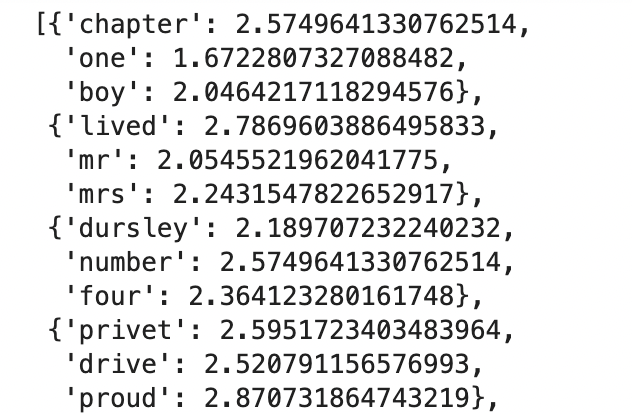
\includegraphics[width=0.9\linewidth]{txt2vector.png}
        \caption{Words converted into vector}
        \label{fig:enter-label}
    \end{minipage}%
    \begin{minipage}{0.5\textwidth}
        \centering
        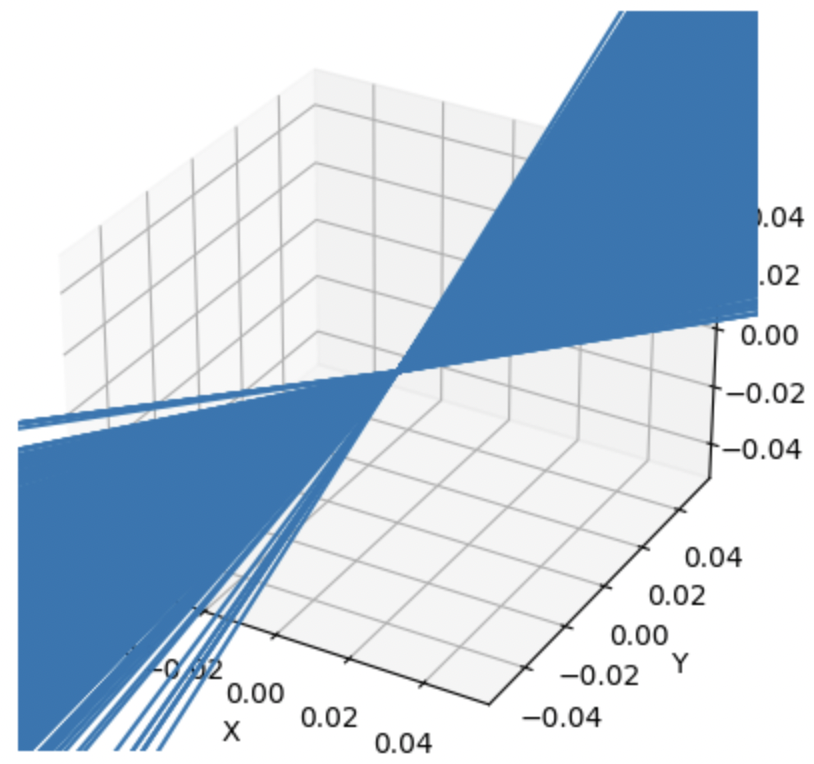
\includegraphics[width=0.9\linewidth]{VecPlot.png}
        \caption{Word Vectors in 3d plane}
        \label{fig: Word Vectors in 3d plane}
    \end{minipage}
\end{figure}

\subsection{Approach-3 (Word2Vec)}
\subsubsection{Understanding Model}
\begin{itemize}
    \item Just like any other nlp model first remove stopwords and tokenize the text.
    \item In my approach i've created map b/w tokens and indices and vice versa. So that conversion becomes easy. 
    \item Since our tokens are strings so we need to encode them for encoding i'm using Approach-1 (\ref{subsec:approach-1}).
    \item In Word2Vec we loop through each word in sentence. in each loop we look at the words left and right of the input word. To make sense of context.
    \item Now consider we have 4 words in the corpus. Now to embed it we will multiply the vector representation of words through \ref{subsec:approach-1} with the weights matrices.
    $$
    \begin{pmatrix}
1 & 0 & 0 & 0\\
0 & 0 & 0 & 1\\
0 & 0 & 1 & 0\\
. & . & . & .\\
. & . & . & .\\
\end{pmatrix}
\times 
\begin{pmatrix}
3 & 1 & 7\\
2 & 9 & 6\\
1 & 0 & 4\\
9 & 1 & 3\\
\end{pmatrix}
=
\begin{pmatrix}
3 & 1 & 7\\
9 & 1 & 3\\
1 & 0 & 4\\
. & . & .\\
. & . & .\\
. & . & .\\
\end{pmatrix}
    $$
    $$
    input \ vector\  \times \ weight\ = \ embeddings
    $$
in embedding we are converting $\mathbb{R}^{4} \rightarrow \mathbb{R}^{3}$.
\item Second layer recieves as input the embeddings, then from it outout is generated $\mathbb{R}^{3} \rightarrow \mathbb{R}^{4}$.
$$
    embeddings\  \times \ weight\ = \ probability\ vector
$$
\item after finding probability vector we need to find context prediction i.e which words are likely to be in the window of the input word.
$$
softmax(probability\ vector) = predicition 
$$
\end{itemize}

\subsubsection{Vector to Similarity Score}
Since I've represented words as vectors and have plotted them. The easiest way to find the similarity score is to check the distance between two vectors. To simplify this I'm \textbf{using Cosine Similarity since Euclidean distances is an expensive task to run}. 
\begin{itemize}
    \item In Cosine similarity focus is on the direction of the vectors, not their magnitude.
    \item If two vectors are on the same side they are similar.
    $$
    Similarity = \frac{\vec{v_1}.\vec{v_2}}{||\vec{v_1}|| \times ||\vec{v_2}||}
    $$
\end{itemize}


\subsection{Findings}    

\begin{figure}[htbp]
    \begin{minipage}{0.5\textwidth}
        \centering
        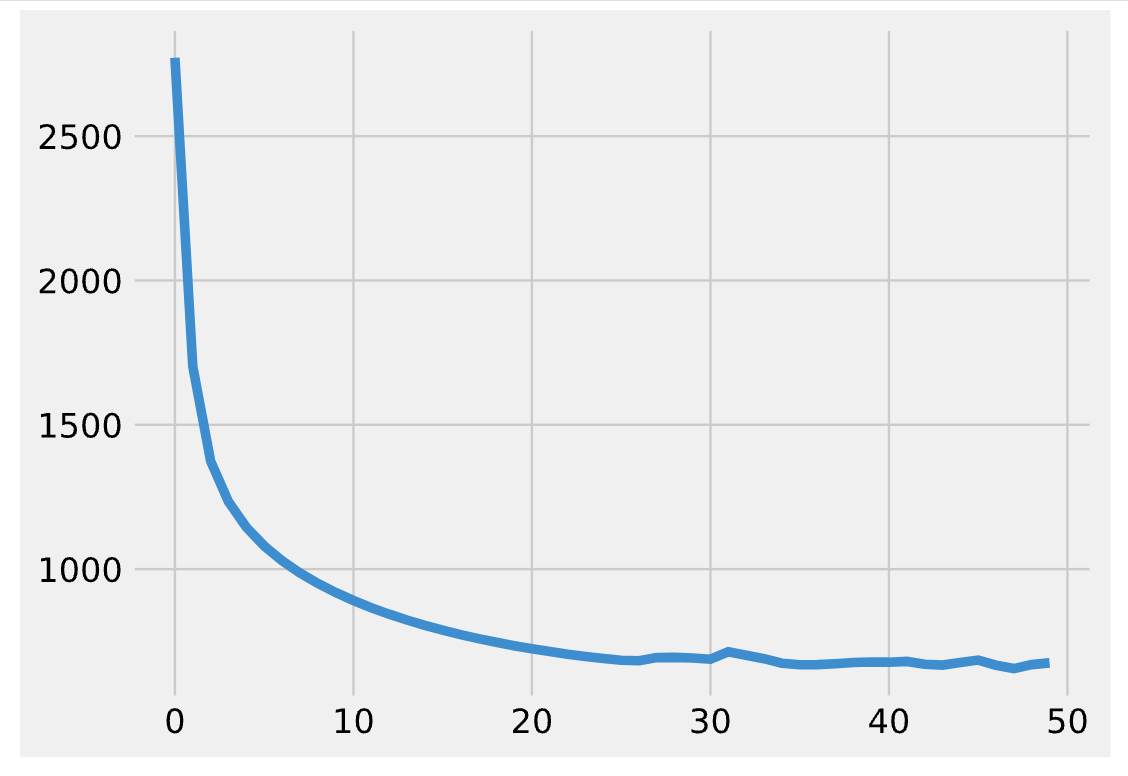
\includegraphics[width=0.9\linewidth]{error after training.png}
        \caption{Error after 50 iterations}
        \label{fig:enter-label}
    \end{minipage}%
\end{figure}

\begin{figure}[htbp]
    % \begin{minipage}{0.5\textwidth}
        \centering
        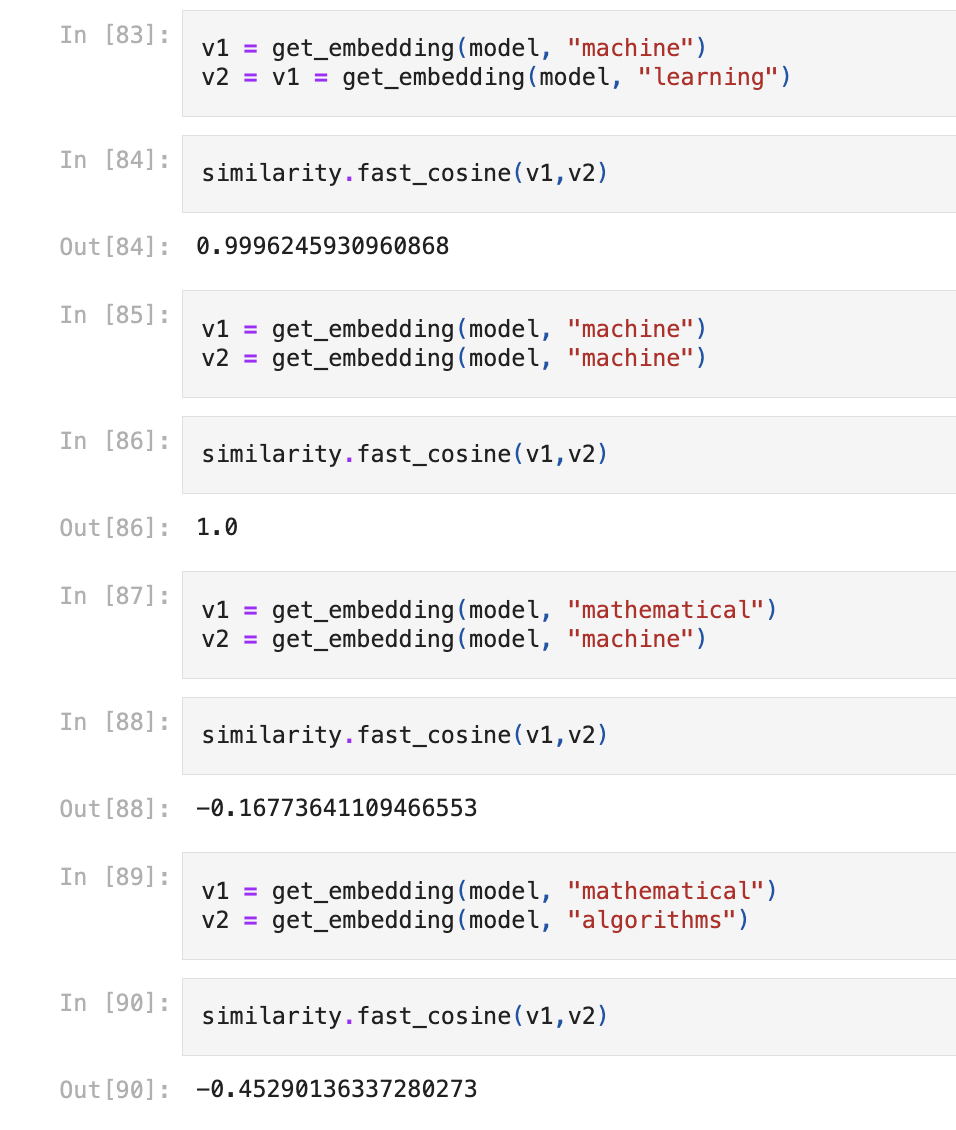
\includegraphics[width=0.5\linewidth]{task1_Untrained_demo.png}
        \caption{Error after 50 iterations}
        \label{fig:enter-label}
    % \end{minipage}%
\end{figure}

\newpage
\subsection{Insights}
\begin{itemize}
    \item If we just convert words to vectors and then find the cosine similarity between them as an idea to find the similarity that would give false results.
    For example: if I just use tf\_idf vectors and apply cosine similarity then the result would be same for each sentence.
    \item Also in Word2Vec approach we see that for each word it uses words before and after that word to make context. \textbf{So if some words are randomly written and we train our model on that than we would find that the output given will be very wrong.}
    \item Also we observe that most of the python libraries like \textbf{spaCy}, \textbf{nltk} are not able to predict the similarity score if those words were not present in the training dataset. $\implies$ \textbf{nltk and spaCy doesn't use supervised learining but rather goes with pseudo-unsupervised/ unsupervised learing for predicting similarity.}
\end{itemize}


\newpage

\section{Phrase and Sentence Similarity}
\textbf{Aim:} Given labeled data-set splitted into training, testing, dev. we have to predict the Phrase and sentence similarity.
\subsection{Approach}
\begin{itemize}
    \item Altough the labelled data was given. But i've used unsupervided learning in this task.
    \item I'm using the frequency of how many pairs have similarity in the training data as my threshold frequency. And calculating if test pairs have similarity score $>$ threshold or not.
    \item Doing this would always give the similarity score to be 1. Because in the dataset{\cite{paws2019naacl}} each pair sentences are just paraphrased.\\
\end{itemize}

\subsection{Insights}
\begin{itemize}
    \item \textbf{for example:} consider these 2 sentences{\cite{paws2019naacl}} to follow the approch mentioned above.\\
    \textbf{Sentence1 -} In Paris , in October 1560 , he secretly met the English ambassador , Nicolas Throckmorton , asking him for a passport to return to \textbf{England through Scotland}.\\
    \textbf{Sentence2 -} In October 1560 , he secretly met with the English ambassador , Nicolas Throckmorton , in Paris , and asked him for a passport to return to \textbf{Scotland through England} .

    \item In the above example all the things are same except the highlighted part. As discussed in the \textbf{Task1} that for a given word word2vec looks at words before and after to make context of the words. Due to this reason the model can't tell the difference between the two sentences.
    
    \item Now consider these examples{\cite{paws2019naacl}}:\\
    \textbf{Sentence1 -} This was a series of nested \textbf{angular standards} , so that measurements in azimuth and elevation could be done directly in polar coordinates relative to the ecliptic .\\
    \textbf{Sentence2 -} This was a series of nested \textbf{polar scales} , so that measurements in azimuth and elevation could be performed directly in angular coordinates relative to the ecliptic .\\

    \item Over here the difference is pretty big but the model wan't able to identify the dissimilarity in these sentences. \textbf{So to tackle situations like this I also add a check to compare Parts of Speech for both Sentences}. 
    
\end{itemize}

\subsection{Findings}
\begin{itemize}
    \item To improve the accuracy of the model we need to shift from unsupervised to supervised learning.
    \begin{figure}[ht]
        \centering
        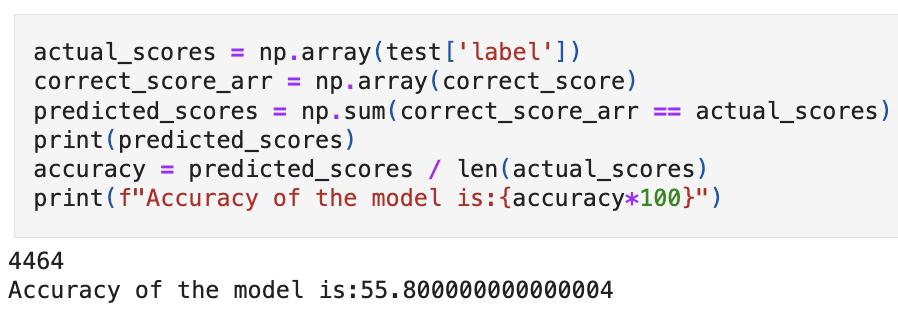
\includegraphics[width=1\linewidth]{accuracy.png}
        \caption{Accuracy of the model}
        \label{fig:enter-label}
\end{figure}
\end{itemize}

\end{document}
